\documentclass[journal,12pt,twocolumn]{IEEEtran}

\usepackage{setspace}
\usepackage{gensymb}
\singlespacing
\usepackage[cmex10]{amsmath}

\usepackage{amsthm}

\usepackage{mathrsfs}
\usepackage{txfonts}
\usepackage{stfloats}
\usepackage{bm}
\usepackage{cite}
\usepackage{cases}
\usepackage{subfig}

\usepackage{longtable}
\usepackage{multirow}

\usepackage{enumitem}
\usepackage{mathtools}
\usepackage{steinmetz}
\usepackage{tikz}
\usepackage{circuitikz}
\usepackage{verbatim}
\usepackage{tfrupee}
\usepackage[breaklinks=true]{hyperref}
\usepackage{graphicx}
\usepackage{tkz-euclide}

\usetikzlibrary{calc,math}
\usepackage{listings}
    \usepackage{color}                                            %%
    \usepackage{array}                                            %%
    \usepackage{longtable}                                        %%
    \usepackage{calc}                                             %%
    \usepackage{multirow}                                         %%
    \usepackage{hhline}                                           %%
    \usepackage{ifthen}                                           %%
    \usepackage{lscape}     
\usepackage{multicol}
\usepackage{chngcntr}

\DeclareMathOperator*{\Res}{Res}

\renewcommand\thesection{\arabic{section}}
\renewcommand\thesubsection{\thesection.\arabic{subsection}}
\renewcommand\thesubsubsection{\thesubsection.\arabic{subsubsection}}

\renewcommand\thesectiondis{\arabic{section}}
\renewcommand\thesubsectiondis{\thesectiondis.\arabic{subsection}}
\renewcommand\thesubsubsectiondis{\thesubsectiondis.\arabic{subsubsection}}


\hyphenation{op-tical net-works semi-conduc-tor}
\def\inputGnumericTable{}                                 %%

\lstset{
%language=C,
frame=single, 
breaklines=true,
columns=fullflexible
}
\begin{document}

\newcommand{\BEQA}{\begin{eqnarray}}
\newcommand{\EEQA}{\end{eqnarray}}
\newcommand{\define}{\stackrel{\triangle}{=}}
\bibliographystyle{IEEEtran}
\raggedbottom
\setlength{\parindent}{0pt}
\providecommand{\mbf}{\mathbf}
\providecommand{\pr}[1]{\ensuremath{\Pr\left(#1\right)}}
\providecommand{\qfunc}[1]{\ensuremath{Q\left(#1\right)}}
\providecommand{\sbrak}[1]{\ensuremath{{}\left[#1\right]}}
\providecommand{\lsbrak}[1]{\ensuremath{{}\left[#1\right.}}
\providecommand{\rsbrak}[1]{\ensuremath{{}\left.#1\right]}}
\providecommand{\brak}[1]{\ensuremath{\left(#1\right)}}
\providecommand{\lbrak}[1]{\ensuremath{\left(#1\right.}}
\providecommand{\rbrak}[1]{\ensuremath{\left.#1\right)}}
\providecommand{\cbrak}[1]{\ensuremath{\left\{#1\right\}}}
\providecommand{\lcbrak}[1]{\ensuremath{\left\{#1\right.}}
\providecommand{\rcbrak}[1]{\ensuremath{\left.#1\right\}}}
\theoremstyle{remark}
\newtheorem{rem}{Remark}
\newcommand{\sgn}{\mathop{\mathrm{sgn}}}
\providecommand{\abs}[1]{\vert#1\vert}
\providecommand{\res}[1]{\Res\displaylimits_{#1}} 
\providecommand{\norm}[1]{\lVert#1\rVert}
%\providecommand{\norm}[1]{\lVert#1\rVert}
\providecommand{\mtx}[1]{\mathbf{#1}}
\providecommand{\mean}[1]{E[ #1 ]}
\providecommand{\fourier}{\overset{\mathcal{F}}{ \rightleftharpoons}}
%\providecommand{\hilbert}{\overset{\mathcal{H}}{ \rightleftharpoons}}
\providecommand{\system}{\overset{\mathcal{H}}{ \longleftrightarrow}}
	%\newcommand{\solution}[2]{\textbf{Solution:}{#1}}
\newcommand{\solution}{\noindent \textbf{Solution: }}
\newcommand{\cosec}{\,\text{cosec}\,}
\providecommand{\dec}[2]{\ensuremath{\overset{#1}{\underset{#2}{\gtrless}}}}
\newcommand{\myvec}[1]{\ensuremath{\begin{pmatrix}#1\end{pmatrix}}}
\newcommand{\mydet}[1]{\ensuremath{\begin{vmatrix}#1\end{vmatrix}}}
\numberwithin{equation}{subsection}
\makeatletter
\@addtoreset{figure}{problem}
\makeatother
\let\StandardTheFigure\thefigure
\let\vec\mathbf
\renewcommand{\thefigure}{\theproblem}
\def\putbox#1#2#3{\makebox[0in][l]{\makebox[#1][l]{}\raisebox{\baselineskip}[0in][0in]{\raisebox{#2}[0in][0in]{#3}}}}
     \def\rightbox#1{\makebox[0in][r]{#1}}
     \def\centbox#1{\makebox[0in]{#1}}
     \def\topbox#1{\raisebox{-\baselineskip}[0in][0in]{#1}}
     \def\midbox#1{\raisebox{-0.5\baselineskip}[0in][0in]{#1}}
\vspace{3cm}
\title{ EE3900 : Assignment-4}
\author{Nelakuditi Rahul Naga - AI20BTECH11029}
\maketitle
\newpage
\bigskip
\renewcommand{\thefigure}{\theenumi}
\renewcommand{\thetable}{\theenumi}
Download all python codes from 
\begin{lstlisting}
https://github.com/Rahul27n/EE3900/blob/main/Assignment_4/Assignment_4.py
\end{lstlisting}
%
and latex-tikz codes from 
%
\begin{lstlisting}
https://github.com/Rahul27n/EE3900/blob/main/Assignment_4/Assignment_4.tex
\end{lstlisting}
\vspace{0.5cm}
\section{QUESTION: LINEAR FORMS Q2.18}
Find the equation of a line that cuts off equal intercepts on the coordinate axes and passes through the point $\myvec{2 \\ 3}$.
\section{SOLUTION}
The general equation of a line can be written as :
\begin{align}
\vec{n}^T\vec{x}=c \label{eq:1}  
\end{align}
where $\vec{n}$ is the normal to the line.

Let the line \eqref{eq:1} cut the x and y co-ordinate axes at $\vec{A}$ and $\vec{B}$ respectively. They can be written as :
\begin{align}
\vec{A} &= \myvec{k \\ 0}\\
\vec{B} &= \myvec{0 \\ k}
\end{align}
where $k$ is a constant, as it is given that the line cuts off equal intercepts on the co-ordinate axes. Hence, the direction vector of this line , say $\vec{m}$ is given by:
\begin{align}
\vec{m} &= \vec{A} - \vec{B}\\
\vec{m} &= \myvec{k \\ 0} - \myvec{0 \\ k}\\
\vec{m} &= \myvec{k \\ -k}
\end{align}
which is equivalent to:
\begin{align}
\vec{m} &= \myvec{1 \\ -1}   
\end{align}
Now the normal vector $\vec{n}$ which is perpendicular to $\vec{m}$ is given by:
\begin{align}
\vec{n} &= \myvec{0 & -1 \\ 1 & 0}\vec{m}\\
\vec{n} &= \myvec{0 & -1 \\ 1 & 0}\myvec{1 \\ -1}\\
\vec{n} &= \myvec{1 \\ 1}\label{eq:2}
\end{align}
Hence from \eqref{eq:1} and \eqref{eq:2} , the equation of the line is given by:
\begin{align}
\myvec{1 & 1}\vec{x}=c\label{eq:3}
\end{align}
It is given that $\myvec{2 \\ 3}$ lies on the line. Hence from \eqref{eq:3} we have:
\begin{align}
c &=\myvec{1 & 1}\myvec{2 \\ 3}\\
c &= 5
\end{align}
Therefore the equation of the line is:
\begin{align}
\myvec{1 & 1}\vec{x}=5
\end{align}
The illustration of the line is shown below :
\begin{figure}[!ht]
       \centering
    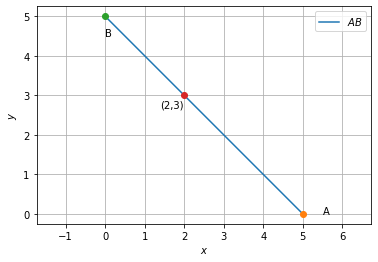
\includegraphics[width=\columnwidth] {Assignment_4_Fig_1.png}
    \caption{Line $\vec{AB}$ making equal intercepts on co-ordinate axes}
    \label{Line AB}
\end{figure}

\end{document}